\documentclass[12pt,a4paper,twoside,openright,italian]{book} % PER ITALIANO
%\documentclass[12pt,a4paper,twoside,openright,italian]{book} % PER INGLESE
\pagestyle{plain}

\usepackage[italian]{babel} %PER ITALIANO
%\usepackage[english]{babel} %PER INGLESE
\usepackage[T1]{fontenc}
%\usepackage[latin9]{inputenc} % PER WINDOWS
\usepackage[utf8]{inputenc} % PER LINUX


\usepackage{url}
\usepackage{amsmath}
\usepackage{graphicx}
\usepackage{setspace}
\usepackage{amssymb}
\usepackage{hyperref}
\usepackage{color}
\usepackage{graphicx}
\usepackage{multicol}
\usepackage {fancyhdr}
\usepackage{geometry}
\usepackage{natbib}
\usepackage{lipsum}
\usepackage{caption}
\usepackage{blindtext}
\usepackage[lined,boxed,commentsnumbered,linesnumbered]{algorithm2e}
\usepackage{listings}
\usepackage{color}
\renewcommand{\ttdefault}{cmtt}

\usepackage[lighttt]{lmodern}

\usepackage{bchart}

\usepackage{wrapfig}

\usepackage[lf]{Baskervaldx} % lining figures
\usepackage[bigdelims,vvarbb]{newtxmath} % math italic letters from Nimbus Roman
\usepackage[cal=boondoxo]{mathalfa} % mathcal from STIX, unslanted a bit
\renewcommand*\oldstylenums[1]{\textosf{#1}}

\linespread{1.1} % Line spacing

%\geometry{a4paper, tmargin=3cm, bmargin=3.5cm, lmargin=3cm, rmargin=3cm} %margini
%\geometry{a4paper, bmargin=4cm} %margini
\geometry{a4paper, bmargin=4cm, lmargin=3.1cm, rmargin=3.2cm} %margini

\newcommand{\noun}[1]{\textsc{#1}}
\newcommand{\whitepage}{\newpage\thispagestyle{empty}\mbox{}}

\graphicspath{{images/}} % Specifies the directory where pictures are stored

\begin{document}

\begin{spacing}{0.90}
\begin{center}
{\Large \thispagestyle{empty}}{
\includegraphics[scale=0.18]{unicalogo}}\par
\end{center}
\end{spacing}

\noindent 
\begin{center}
\vspace{0.7cm}
\textbf{\noun{\Large UNIVERSIT\`A DEGLI STUDI DI CAGLIARI}}\par
\end{center}{\LARGE \par}

\noindent 
\begin{center}
\textbf{\large FACOLT\`A DI SCIENZE}\par
\end{center}{\large \par}

\noindent
\begin{center}
%{\large Corso di Laurea Magistrale in Informatica}\par  % PER MAGISTARLE
{\large Corso di Laurea Triennale in Informatica}\par  % PER TRIENNALE
\end{center}{\large \par}

\vspace{2.6cm}


\begin{center}
\textbf{\LARGE Analisi empirica di Litecoin}\par
\end{center}{\LARGE \par}


\begin{spacing}{0.90}
\vspace{3.7cm}
\textbf{\large Relatore}{\large \hfill{}}\textbf{\large Studente}{\large \par}
\end{spacing}

{\large Prof. Massimo Bartoletti\hfill{}Giulia Argiolas~}{\large \par}

\begin{spacing}{0.90}
{\large \hfill{}Matr. N. 65385}{\large \par}
\end{spacing}

\vspace{2.5cm}


\begin{center}
ANNO ACCADEMICO 2017/2018\par 
\end{center}

\whitepage
\whitepage

\vspace{4cm}
La tesi ha come obiettivo l'analisi della blockchain Litecoin con i presupposti di un confronto con Bitcoin. Introduce Litecoin, caratteristiche e differenze con Bitcoin, utilizzi presenti e prospettive future e contiene delle analisi svolte tramite l’estensione e l’utilizzo del tool BlockAPI, già operativo per le blockchain Bitcoin ed Ethereum, relative alla distribuzione dell’hashing power tra i mining pools, il mining di blocchi vuoti, la diffusione del merged mining e l’utilizzo dell’OP\_RETURN per segnalare l’adesione a protocolli o servizi.

\whitepage

\frontmatter
	\tableofcontents

\mainmatter
\chapter{Introduzione}

\section{Obiettivi}
L’obiettivo è lo studio della blockchain di Litecoin per effettuare una comparazione con Bitcoin. A tal fine ho svolto delle analisi riguardanti prevalentemente il lato tecnologico di essa, lo sviluppo, le applicazioni, ma anche il lato economico, tramite dati esterni, come fees, exchange rates e la loro evoluzione nel tempo.
\section{Contributi}
Per l’analisi della blockchain Litecoin ho esteso il tool BlockAPI, implementando le strutture dati e le queries necessarie a tal fine. La parte tecnica dell’estensione del tool verrà discussa nel capitolo 2.
\section{Struttura della tesi}
La tesi presenta un background tecnico iniziale necessario a capire Bitcoin e valido per tutte le criptovalute da esso derivate e mostra le caratteristiche principali per cui Litecoin differisce da Bitcoin. Segue un’introduzione delle tecnologie utilizzate e del mio contributo al tool che è stato utilizzato per l’analisi. Infine le analisi, per ciascuna delle quali viene illustrato un contesto per comprenderla, lo svolgimento di essa, il codice e le queries ed i risultati numerici e loro eventuali rappresentazioni grafiche.

\section{Background}
\subsection{Bitcoin}
Bitcoin è una criptovaluta nata nel 2009 ad opera di Satoshi Nakamoto, la cui vera identità è ancora ignota. Open source, orientata all’anonimato, decentralizzata e peer to peer, non possiede alcun server “centrale” o organismo di controllo. È una risorsa totalmente virtuale che non prevede un’unità fisica associata: i Bitcoin sono “coniati” tramite un processo, il cosiddetto mining, che comporta una competizione nel cercare le soluzioni di un problema computazionale estremamente oneroso da risolvere ma la cui soluzione sia semplicissima da verificare, detto Proof of Work.
Chiunque può minare tramite la potenza di calcolo di cui dispone, ma la difficoltà del puzzle crittografico viene ricalcolata ogni 2016 blocchi -approssimativamente 2 settimane- in base alla potenza di calcolo del network affinché in media un blocco di transazioni sul network venga generato e validato ogni 10 minuti. Dunque ogni 10 minuti circa un nuovo blocco viene confermato e aggiunto alla blockchain e questo lavoro viene ricompensato con una quantità prestabilita di Bitcoin nuovi di zecca. 
La ricompensa per il miner si dimezza circa ogni 4 anni perché, dal momento che il protocollo Bitcoin permette l’esistenza di massimo 21 milioni di unità monetarie, la ricompensa deve essere sufficientemente elevata da incentivare il lavoro del miner ma non così tanto da deprezzare la valuta mettendo in circolazione prematuramente un numero eccessivo di Bitcoin. Attualmente la ricompensa ammonta a 12.5 BTC e nel 2020 subirà un nuovo dimezzamento.\cite{blockonomi}
Le informazioni e lo storico di tutte le transazioni sulla rete sono immutabili e distribuiti sui nodi che la costituiscono. La struttura dati atta a garantire ciò è la Blockchain e tramite essa Bitcoin decentralizza e distribuisce sulla rete le funzioni di emissione di valuta (mining) e di compensazione (halving) eliminando la necessità di una banca centrale.



\subsubsection{Background tecnico}
Per capire Bitcoin è utile chiarire cosa sia effettivamente una transazione in Bitcoin e in cosa differisca da una “ordinaria”, ad esempio con carta di credito. Il concetto di transazione bancaria che conosciamo prevede una privacy ferrea e l’utilizzo della crittografia al fine di non far intercettare dati sensibili ai malintenzionati, mentre in questo caso la transazione è pubblicamente disponibile per intero in un registro pubblico immutabile e non contiene dati personali. Bitcoin ha praticamente trasformato i soldi in una struttura dati e fatto in modo che sia quasi impossibile per chiunque creare una transazione illeggittima, ma che allo stesso tempo sia facilissimo verificarne la validità. Una transazione è infatti una struttura dati che codifica e trasferisce un valore da una fonte di fondi, detta input, ad una destinazione, detta output. La tabella 1.1 riporta la struttura dell'header di una transazione.

\begin{table}[ht]
	\centering
	\resizebox{\textwidth}{!}{
\begin{tabular}{|c|c|c|}
\hline
\textbf{	 
	Dimensione }&\textbf{ Campo }&\textbf{ Descrizione }\\ \hline
 
	 
4 Bytes	& Versione & Specifica quali regole segue la transazione \\ \hline
 
	 
1-9 Bytes (VarInt)	& Input Counter &  Quanti input sono inclusi\\ \hline
 
Variable	& Inputs &  Uno o più input di transazione\\ \hline
 	 
1-9 Bytes (VarInt)	& Output Counter &  Quanti output sono inclusi \\ \hline
 	 
Variable	& Outputs &  Uno o più input di transazione\\ \hline
 	 
4 Bytes	& Locktime & Un Unix timestamp o numero del blocco \\ \hline
\end{tabular}}
\caption{Struttura dell'header di una transazione Bitcoin \cite{masteringbitcoin}}
\end{table}


I componenti di una transazione sono i cosiddetti UTXO, o input di transazione non spesi, la cui aggregazione dà il “saldo” dell’utente -in Bitcoin non esiste un vero e proprio concetto di saldo- e il resto di un UTXO più grande del valore desiderato viene restituito, in modo analogo, come UTXO più piccolo (che assume il valore del resto). 
Ogni transazione Bitcoin contiene almeno un input e output, ad eccezione delle transazioni coinbase che contengono un solo output del valore della ricompensa per il miner, già precedentemente accennata. Tutti gli outputs ad eccezione dei cosiddetti OP\_RETURN producono a loro volta bitcoin spendibili e sono composti da un importo in bitcoin e un “locking script” che ha la funzione di verifica: solo chi soddisfa le condizioni poste dallo script può riscattare l’output. La transazione viene firmata tramite la chiave privata del proprietario e può essere sbloccata solo dall’indirizzo del destinatario legittimo.
Chiunque voglia ricevere un pagamento, o effettuarne uno, necessita di una copia pubKey:privateKey.Ogni partecipante al network crea tramite il client una privateKey di 256 bit che occorrerà per firmare la transazione.
Da questa chiave si genera successivamente la pubKey di 512 bit, tramite l’algoritmo ECDSA su curva ellittica secp256k1.
Tale chiave verrà usata per la verifica dell'autenticità della firma digitale del mittente.  
Per sicurezza e praticità si esegue un doppio hash: per prima cosa si calcola SHA-256(PubKey), e successivamente si esegue RIPEMD-160(SHA-256(PubKey)); per ottenere l'indirizzo si utilizza una ulteriore codifica in Base58Check per ottenere un indirizzo in formato standard.


\begin{figure}[h!]
\centering
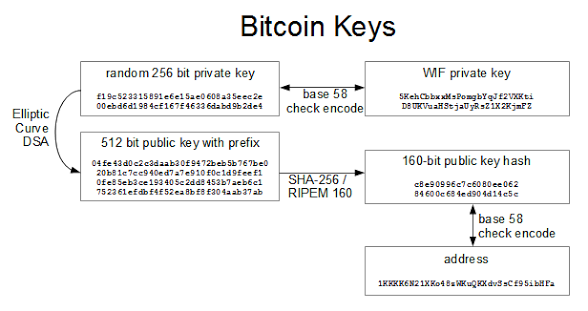
\includegraphics[width=0.9\linewidth]{EcdsaToAddress-bstavroulakis}
\caption{Processo di codifica di un indirizzo bitcoin}
\label{fig:ecdsatoaddress-bstavroulakis}
\footnote{Fonte:bstavroulakis.com}
\end{figure}


Ogni transazione validata dal network viene inserita in un blocco di transazioni che è accodato alla blockchain.
La blockchain è un registro pubblico e distribuito che tiene traccia di tutte le transazioni che sono state effettuate fin dal primo blocco. È immutabile e ciascun nodo ne contiene una copia: ai fini di questa tesi non è necessario dettagliare il sistema di consenso (la Proof of Work precedentemente citata) ma è fondamentale ricordare che l’intero sistema si basa su di esso e, soprattutto, che la versione “ufficiale” della blockchain è quella su cui il maggior numero di nodi sono d’accordo. Ciò che rende estremamente sicura la blockchain è proprio l’utilizzo della curva ellittica in associazione alle funzioni di hashing precedentemente citate, SHA-256 e RIPEMD-160, che processano l’input X producendo in output una stringa di lunghezza fissa H(X) da cui non poter ricavare l’input originario X. Inoltre, minime variazioni di X possono portare variazioni enormi in H(X) ed essa non deve contenere una pre-immagine di X.

\begin{figure}[h!]
\centering
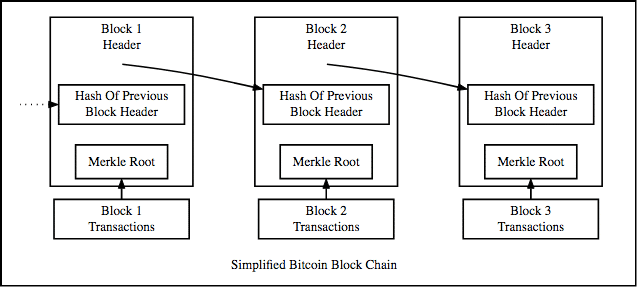
\includegraphics[width=1.0\linewidth]{SimplifiedBlockchainBlockGeeks}
\caption{Struttura semplificata di una blockchain}
\label{fig:simplifiedblockchainblockgeeks}
\footnote{Fonte blockgeeks.com}
\end{figure}


La blockchain è una lista concatenata che contiene dati e un hash pointer che punta al blocco precedente. Un hash pointer differisce da un normale puntatore perché invece di limitarsi a contenere l’indirizzo del blocco precedente contiene anche l’hash dei dati del blocco che punta. Nel caso di Bitcoin, inoltre, la funzione di hashing viene applicata doppiamente nell’header in due casi.\\

% \usepackage[table]{xcolor} is necessary !
\begin{table}[ht]
	\centering
	\resizebox{\textwidth}{!}{
\begin{tabular}{|c|c|c|c|}
	\hline
	\textbf{Bytes} &       \textbf{Name}        & \textbf{Data Type} &                     \textbf{Description}                     \\ \hline
	      4        &          version           &      int32\_t      &   Indica il set di regole utilizzato per la validazione del blocco.   \\ \hline
	      32       & previous block header hash &      char[32]      &            Hash dell'header del blocco precedente           \\ \hline
	      32       &      merkle root hash      &      char[32]      &                Hash in internal byte order derivato dagli hash delle transazioni.                \\ \hline
	      4        &            time            &     uint32\_t      & Unix timestamp del momento in cui il miner ha iniziato l'hashing dell'header \\ \hline
	      4        &           nBits            &     uint32\_t      &  
	      Codifica del valore target per la validazione dell'hash\\ \hline
	      4        &           nonce            &     uint32\_t      & 
	      Numero arbitrario, modificabile dal miner per rispettare nBits \\ \hline
\end{tabular}}
\caption{Struttura dell'header di un blocco Bitcoin (documentazione ufficiale bitcoin.org)}
\end{table}


Nella tabella 1.2 possiamo osservare la struttura degli 80 Bytes dell’header di ciascun blocco. Tenendo presente quanto affermato in precedenza sulle funzioni di hashing risulta chiara la virtuale impossibilità di riuscire ad effettuare qualsivoglia modifica senza che questa abbia un impatto sull’intera blockchain.

\begin{figure}
	\centering
	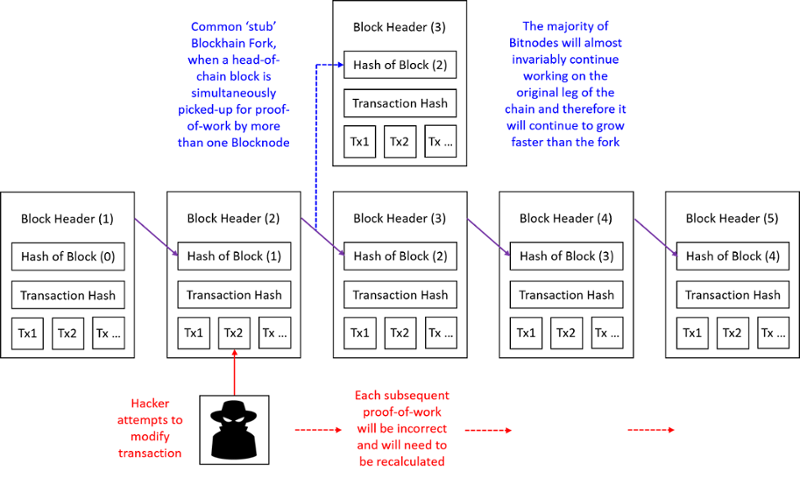
\includegraphics[width=1.0\linewidth]{images/blockchain-diagram}
	\caption{Impatto della modifica di una transazione sulla blockchain: ogni proof-of-work successiva risulterà scorretta e necessiterà il ricalcolo, mentre la maggioranza dei nodi continuerà a lavorare sui dati della blockchain corretta.}
	\label{fig:blockchain-diagram}
\end{figure}


È questo a garantire l’inalterabilità del contenuto della blockchain: oltre alla difficoltà data dalla potenza computazionale richiesta per rendere almeno fattibile l’attacco, il costo lo rende nella quasi totalità dei casi insostenibile o non profittevole.
A titolo d’esempio, riporto la stima di quanto costerebbe sferrare un attacco alle principali blockchain allo stato attuale

\begin{figure}[h]
\centering
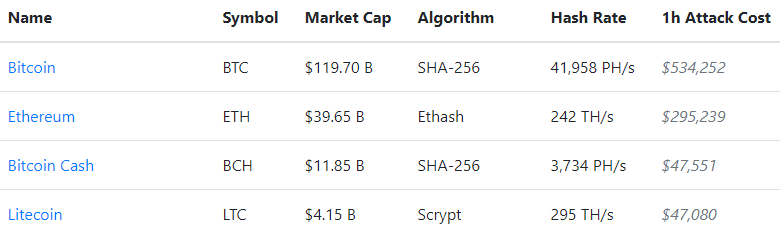
\includegraphics[width=1.0\linewidth]{51cost2therevenge}	
\caption{Costo stimato (02/08/2018) di un attacco alle principali criptovalute}
\label{fig:51cost2therevenge}
\footnote{Fonte: crypto51.app}
\end{figure}



In breve: la blockchain è un registro pubblico immutabile contenente una serie di blocchi di transazioni validate, ognuna delle quali consiste in un trasferimento di fondi da uno o più input non spesi ad uno o più output, e tutto ciò avviene in modo decentralizzato ed è reso sicuro tramite le curve ellittiche e funzioni di hashing che garantiscono che solo i legittimi proprietari possano usufruire dei fondi.



\subparagraph{Forks e Altcoins}

L’esistenza stessa di una blockchain dipende dall’aderenza alle regole dell’intero network. Blocchi che non rispettano le regole non possono essere validati.
Bitcoin, essendo open source, viene mantenuto e valutato da comunità di sviluppatori che reagiscono ai problemi che emergono nel network tramite dei BIP (Bitcoin Improvement Proposal) che formalmente sono uno standard di proposta di miglioramento. Questi possono riguardare il protocollo o le regole. Una soft fork consiste infatti in un cambiamento di protocollo o di regole in modo retrocompatibile: il software continuerà a riconoscere i blocchi precedenti e i vecchi nodi non aggiornati saranno in grado di validare nuovi blocchi. Detta consensus fork, per la sua attuazione è sufficiente che la maggioranza dei miner sia d’accordo. Talvolta si hanno, tuttavia, notizie di attacchi hacker verso i nodi non aderenti (es: DDoS) per forzarne indirettamente l’adesione. Un esempio di soft fork è l’implementazione di SegWit, oggetto di un’analisi al capitolo 4.
Qualora non fosse presente il consenso necessario tra i miners e la nuova versione del software non fosse retrocompatibile si verificherebbe un hard fork: quando ciò si verifica la blockchain subisce una separazione definitiva e il possessore di criptovaluta la possiede ora duplicata sulla blockchain forked.
Un hard fork piuttosto noto di Bitcoin è Bitcoin Cash: differisce dal protocollo originale per la dimensione del blocco, che da 1 passa ad 8 MB. Chi possedeva X bitcoin (BTC) al momento del forking ha potuto ottenere gratuitamente X bitcoincash (BCH).
Infine ci sono le cosiddette altcoins: forks del codice sorgente di Bitcoin, blockchain totalmente separata, differenze di protocollo scarsamente compatibili. Litecoin è definibile a tutti gli effetti una altcoin ed è stata a sua volta oggetto di codebase forks.


\begin{figure}
	\centering
	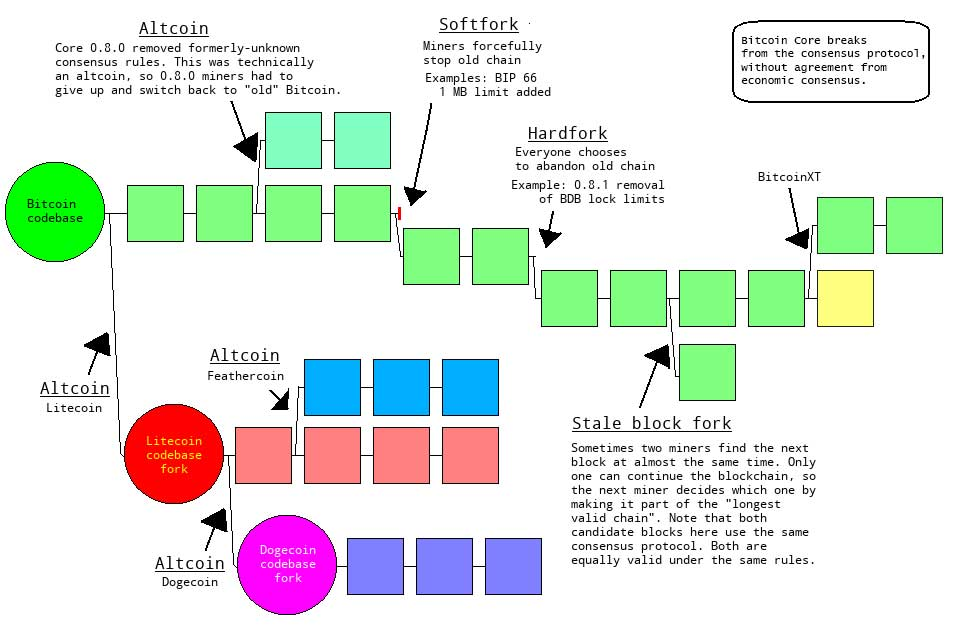
\includegraphics[width=1.0\linewidth]{images/altcoinsoftforksetc}
	\caption{Classificazione delle blockchain derivanti dalla codebase di Bitcoin.}
	\label{fig:altcoinsoftforksetc}
	\footnote{Fonte medium.com}
\end{figure}





\subsection{Litecoin}
Litecoin è una criptovaluta peer to peer che dal punto di vista tecnico condivide gran parte dell’implementazione di Bitcoin. Non è considerabile una fork di Bitcoin in senso stretto poiché non c’è stata la duplicazione della moneta, bensì una source code fork: è stato effettuato il fork del codice sorgente e del client open source Bitcoin Core e sono state effettuate delle modifiche sostanziali che si sono riflesse nella blockchain e le due valute non hanno uno storico comune. 
Nasce nel 2011 ad opera dell’ex ingegnere MIT Charlie Lee, con l’intento dichiarato di diventare rispetto a Bitcoin “ciò che l’argento è rispetto all’oro”; già da questa frase si può comprendere come Litecoin sia una valuta che si presta a micropagamenti e operazioni più rapide rispetto a Bitcoin. Lee sostiene di non aver concepito Litecoin come sostituto di Bitcoin, bensì come complemento per risolvere alcune criticità da lui rilevate.

Pur condividendone per la maggior parte struttura e protocollo presenta alcune differenze fondamentali:

Velocità: nel network Litecoin un blocco viene aggiunto alla Blockchain circa ogni 2.5 minuti contro i 10 di Bitcoin quadruplicando la velocità di creazione dei blocchi. Questo implica la possibilità di confermare le transazioni molto più rapidamente e a costi minori, nonché una minor congestione di rete e una riduzione del pericolo di attacchi double-spending a causa della finestra temporale utile ridotta.
La proof of work utilizza l’algoritmo Scrypt: per ridurre il pericolo di centralizzazione del calcolo nei nodi che possono permettersi hashing powers enormi tramite hardware pre-esistente specializzato per il mining.
Scrypt implementa alcune funzioni che fanno un largo uso di memoria per ridurre drasticamente l’efficienza dei circuiti logici tipici degli ASIC, privi di cache e ottimizzati per il mining intensivo. Trattandosi di un problema memory-hard sono privilegiate grandi quantità di RAM veloce. 
Questa scelta è stata fatta per evitare l’aumento esponenziale della difficoltà di mining in tempi brevi in un mercato in cui cominciavano già a prendere piede i suddetti dispositivi: Litecoin è nato oltre due anni dopo e la centralizzazione sarebbe stata un pericolo concreto.
84 milioni di unità monetarie, il quadruplo rispetto a Bitcoin.

I meccanismi di regolazione della difficoltà e di halving sono analoghi a Bitcoin ma i numeri cambiano: la difficoltà viene ricalcolata ogni 3.5 giorni -4 volte più velocemente- e l’halving è fissato ogni 840.000 blocchi -il quadruplo- in linea con la velocità e il numero di unità monetarie di Litecoin.

\subsubsection{Qualche dato su Litecoin}
Ad agosto 2018 risultano già minati e circolanti 57.000.000 Litecoin su un totale di 84.000.000 e il valore di un LTC fluttua intorno ai 60 euro.

\begin{figure}[h!]
	\centering
	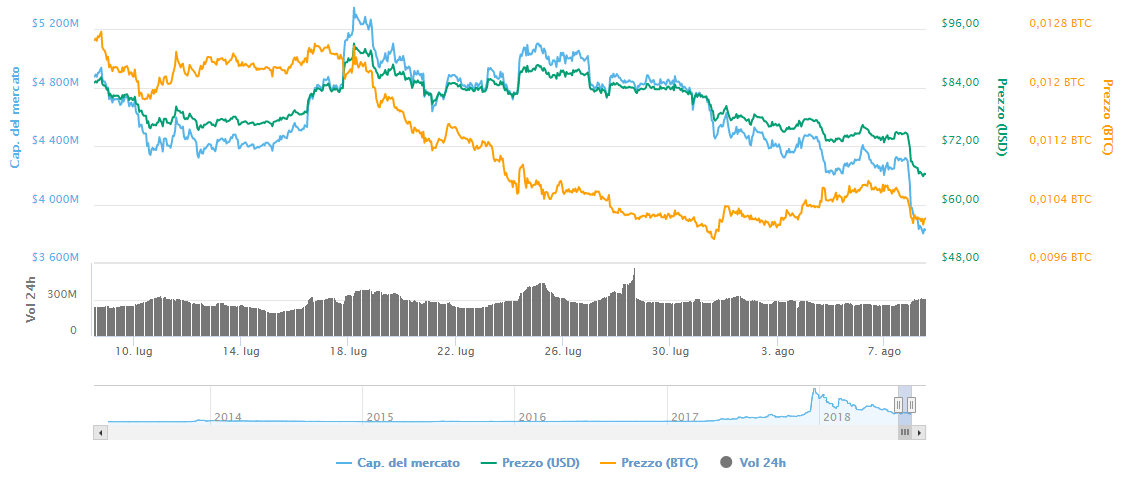
\includegraphics[width=1.0\linewidth]{images/LitecoinCoinMarketCap}
	\caption{Confronto tra gli andamenti di mercato di Bitcoin e Litecoin}
	\label{fig:litecoincoinmarketcap}
	\footnote{Fonte Coinmarketcap.com}
\end{figure}


Questo grafico illustra l’andamento sul mercato di Litecoin ed evidenzia come questo segua tendenzialmente l’andamento di Bitcoin.
Correntemente la difficoltà è prossima al $10^{7}$   \cite{bitcoinwisdom}, la ricompensa per un nuovo blocco ammonta a 25 LTC e il dimezzamento è previsto per il 6 agosto 2019.
La blockchain Litecoin contiene attualmente \~{}1.480.000 blocchi.



\chapter{Tecnologie utilizzate}

\section{BlockAPI: Blockchain analytics API}
BlockAPI è un tool open source in linguaggio Scala che crea un database a partire da una blockchain permettendo di effettuare su di essa analisi tramite query in vari DML. Si appoggia a librerie esterne per ottenere una rappresentazione Java dei dati della blockchain d’interesse e può effettuare richieste Curl tramite API di servizi esterni per accedere a dati non presenti sulla blockchain ma necessari alle analisi: ad esempio per analisi sui bilanci, sulle fees e sui tassi di scambio è utile sapere quanto valeva la criptovaluta analizzata, principalmente in euro o dollari, al momento della transazione e per fare ciò si può ricorrere alle API di Coindesk o Cryptocompare. 
Il tool supporta Bitcoin ed Ethereum, ai quali ho aggiunto Litecoin.\\
\section{Database}
Per effettuare le analisi sulla blockchain Litecoin ho utilizzato il linguaggio SQL e il DBMS MySQL.\\
\section{Analisi}
Per effettuare una specifica analisi occorre innanzitutto costruire il DB con i dati d’interesse per essa (es hash del blocco o delle transazioni, input/output scripts, tipo della transazione): per fare ciò esiste per ogni analisi uno script in Scala che automatizza la creazione di una tabella contenente i dati in questione tramite l’ausilio di librerie di terze parti per il parsing dei dati. 
Tramite i metodi start(block number) e end(block number) è possibile restringere l’analisi a una sezione più o meno estesa della blockchain. Questa possibilità è particolarmente utile quando si analizza una funzionalità implementata con un BIP in un momento preciso oppure se i risultati prima di una determinata data non siano particolarmente significativi. I dati vengono trattati tramite la loro rappresentazione Java fornita dalle librerie precedentemente menzionate, linguaggio con cui Scala si interfaccia agevolmente. Una volta popolate le tabelle tramite l’esecuzione dello script con le informazioni necessarie è possibile effettuare l’analisi vera e propria tramite query eseguibili da command line o GUI sul DBMS scelto. Per tutte le analisi necessarie mi sono avvalsa del client GUI MySQL Workbench.

\section{Connessione con Litecoin}
Per ottenere una rappresentazione Java della blockchain Litecoin è stato necessario utilizzare nel tool le funzionalità di LitecoinJ \cite{litecoinjgithub}, corrispettivo di BitcoinJ per Bitcoin. La libreria permette operazioni standard come deserializzazione, decodifica, decriptazione indirizzi e key.
La connessione avviene tramite l’utilizzo del daemon litecoin in modalità server in modo da poter sfruttare le RPC (Remote Procedure Call) per ottenere i dati da passare al tool.

Per supportare la blockchain Litecoin ho aggiunto al tool le strutture dati necessarie: estendendo le interfacce Blockchain e Block e implementando le funzioni che hanno innanzitutto permesso a BlockAPI di effettuare le chiamate RPC, poi di parsare la risposta per ottenere le informazioni necessarie sulla blockchain, sui blocchi e sulle transazioni.

\subsection{Implementazioni}





\chapter{Analisi}

\lstset{frame=tb,
	language=Scala,
	aboveskip=3mm,
	belowskip=3mm,
	showstringspaces=false,
	columns=flexible,
	basicstyle={\small\ttfamily},
	numbers=none,
	numberstyle=\tiny\color{gray},
	keywordstyle=\color{blue},
	commentstyle=\color{green},
	stringstyle=\color{red},
	breaklines=true,
	breakatwhitespace=true,
	tabsize=3
}

\begin{lstlisting}
// Hello.java
import javax.swing.JApplet;
import java.awt.Graphics;

public class Hello extends JApplet {
	public void paintComponent(Graphics g) {
		g.drawString("Hello, world!", 65, 95);
	}    
}
\end{lstlisting}

\section{Mining pools}

\subsection{Contesto}
Sebbene sia possibile per ogni utente singolo minare criptovalute, l’incremento della difficoltà nel mining lo rende inutile poiché le probabilità di risolvere il puzzle sono minime. Pertanto il mining avviene quasi esclusivamente tramite mining pools che sfruttano la potenza di calcolo aggregata per risolvere il blocco e spartiscono i guadagni tra i partecipanti.


L’hashing power complessivo al momento dell’analisi corrente è circa 275 TeraHashes/s ed è cresciuto esponenzialmente negli ultimi anni: riporto il grafico su scala logaritmica dal 2014 ad oggi e uno zoom in scala lineare dell’andamento nell’ultimo anno.


\begin{figure}[h]
	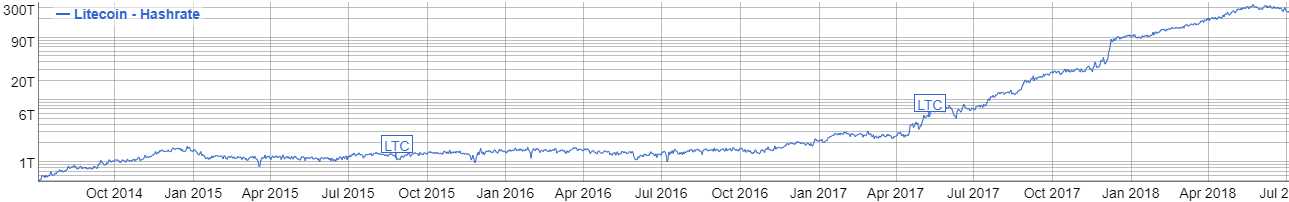
\includegraphics[width=1.0\linewidth]{provahashratelog}
	\caption{}
	\label{fig:provahashratelog}
\end{figure}

\begin{figure}
	\centering
	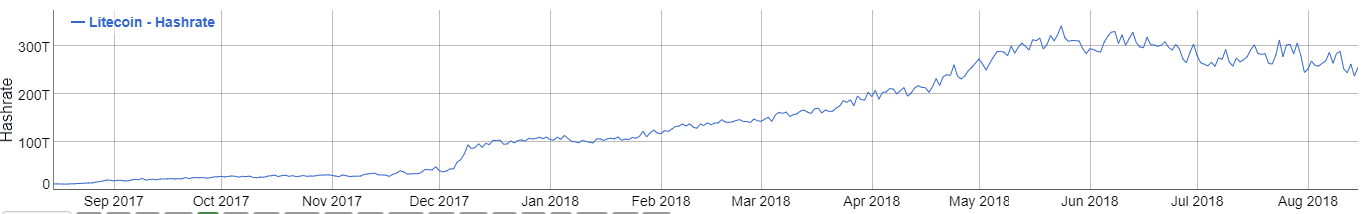
\includegraphics[width=1.0\linewidth]{LitecoinHashRateLIN}
	\caption{}
	\label{fig:litecoinhashratelin}
\end{figure}




[bitinfocharts.com]
La suddivisione riportata in seguito è datata 02/08/2018, è limitatamente indicativa nel tempo e presenta un margine d’errore di qualche punto percentuale: i dati istantanei sulla distribuzione dell’hashing power sulla rete sono molto variabili poiché l’unico modo per ottenerli sono delle stime effettuate sulla base della velocità del network nel processare i nuovi blocchi e delle indicazioni fornite dai pools stessi. Tuttavia la loro osservazione fornisce dati utili per comprendere meglio i risultati delle analisi.


\begin{figure}[h!]
	\centering
	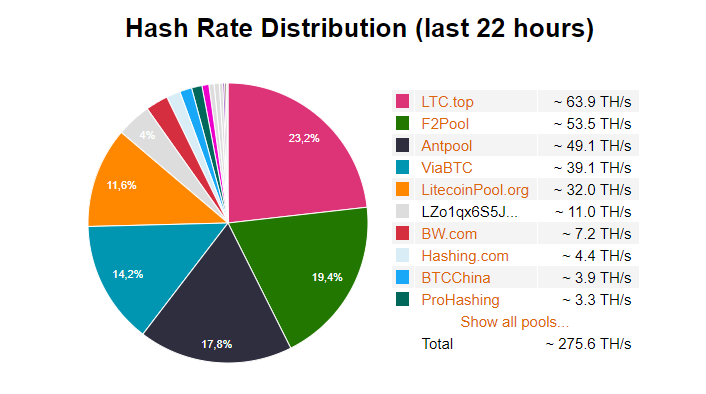
\includegraphics[width=1.0\linewidth]{images/HashingPower020818}
	\caption{dati 02/08/2018 litecoinpool.org}
	\label{fig:hashingpower020818}
\end{figure}


\subsection{Obiettivo dell’analisi}
Verificare la distribuzione del potere di mining nel tempo: ci sono pools che superano il 50\% di hashing power? Per il mantenimento della decentralizzazione della Blockchain è importante che questo non accada perché si configurerebbe il rischio di un cosiddetto 51\% attack: quando qualcuno riesce a disporre di una potenza di calcolo superiore al 50\% del totale, può creare blocchi non rispondenti alle specifiche del protocollo della criptovaluta, tra cui ad esempio blocchi contraffatti con i quali spendere due volte gli stessi token o addirittura impedire ad altri miner di validare il blocco al fine di incassare le reward.


\subsection{Svolgimento}
Ogni nuovo blocco minato contiene una transazione, detta coinbase, che non contiene alcun input ma contiene in output la somma di ricompensa per il blocco minato e fees di tutte le transazioni in esso contenute.
Spesso i mining pools inseriscono nella coinbase un identificatore come una sigla, un codice ascii o non ascii, oppure il proprio nome seguito dal miner per “firmare” il blocco. È sufficiente esaminare tramite visualizzatore esadecimale l’hex della coinbase di un blocco per verificare se è presente un identificatore di questo tipo.

Il tool BlockAPI contiene una lista di identificatori noti per Bitcoin ed Ethereum, ai quali ho aggiunto alcuni identificatori o pattern relativi a mining pools che minano Litecoin oppure sia Bitcoin che Litecoin. 
Dopo la creazione della tabella, viene eseguito il seguente script per popolarla:

\begin{lstlisting}
blockchain.foreach(block => {
txTable.insert(Seq(block.hash.toString(), convertDate(block.date), block.getMiningPool(), block.isMerged()))
})
\end{lstlisting}

Per ogni blocco nell’intervallo selezionato, si inserisce nella tabella l’hash del blocco, il timestamp, il pool che ha minato il blocco e un ulteriore campo relativo al merged mining (che tratterò nelle analisi successive). La funzione getMiningPool() fa parte dell’interfaccia Block, che in questo caso è overrided [?] da getLitecoinPool(txs.head). L’override effettuato per ogni blockchain permette di verificare per ogni criptovaluta la presenza di uno degli identificatori ad essa relativi.


\subsection{Query}

\begin{lstlisting}
SELECT Pool.pool AS Pool, COUNT(*) AS Blocks
FROM myblockchainlite.ltcpools AS Pool
GROUP BY Pool.pool
ORDER BY Blocks DESC;
\end{lstlisting}

\subsection{Risultati}

Su un totale di 312432 blocchi di cui ci è noto il miner, possiamo fare le seguenti osservazioni:

\begin{figure}
	\centering
	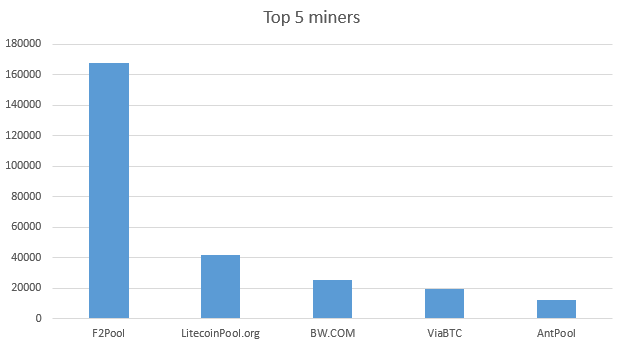
\includegraphics[width=1.0\linewidth]{images/top5miners}
	\caption{}
	\label{fig:top5miners}
\end{figure}


I primi 5 miners hanno complessivamente minato 265756 blocchi. Risulta quindi che l’85\% dell’hashing power dei blocchi di miner noto sia concentrato nei primi 5. 
F2Pool, noto anche come DiscusFish e attivo dal 2013 su BTC, ETH e altre criptovalute, è stato uno dei primi pools importanti ad interessarsi a Litecoin e domina totalmente il computo totale con un impressionante 53.64\% dei blocchi noti della blockchain. Correntemente ha un hashing power che si attesta intorno al 20\% del totale.

\begin{figure}[h!]
	\centering
	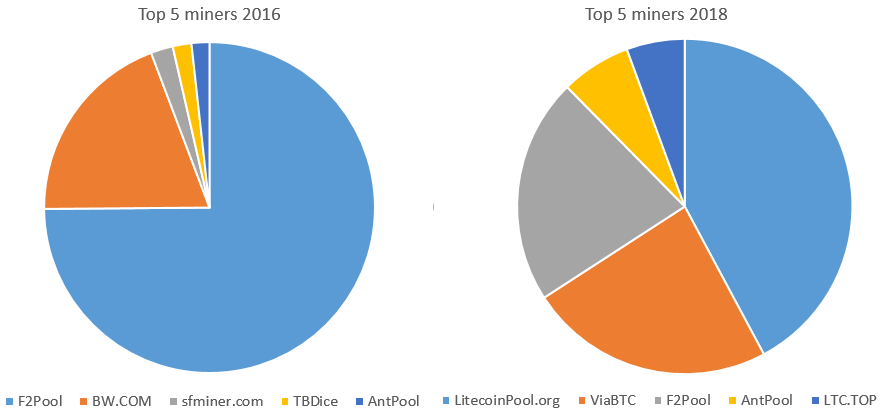
\includegraphics[width=1.0\linewidth]{images/top5miners2016vs2018}
	\caption{}
	\label{fig:top5miners2016vs2018}
\end{figure}



Il confronto tra i dati del 2016 e i dati (ovviamente parziali) del 2018 evidenziano il cambio di distribuzione del mining di Litecoin: se da un lato la maggior distribuzione dei blocchi minati tra i mining pools indica una migliore decentralizzazione, dall’altro evidenzia che i miners indipendenti o i piccoli pools sono praticamente scomparsi a causa dell’aumento della difficoltà, correntemente > 10.000.000.

Infatti se nel 2014 201587 blocchi risultano minati da ignoti su un totale di 215094 (93.7\%) denotando un interesse molto marginale da parte dei mining pools, perlopiù pools già operativi su Bitcoin, e molto maggiore da parte di miners privati, nel 2017 la percentuale scende al 42\% in cui va tenuto conto di margine d’errore dovuto a due cause: la prima, logica, è che potrebbero esserci dei mining pools di cui non si conoscono gli identificatori o non ne usano oppure potremmo non conoscere tutti gli identificatori di ogni mining pool tra quelli già noti, la seconda è che un bug di LitecoinJ nonché della precedente versione di BitcoinJ, sul quale al momento non è possibile intervenire, impedisce il parsing corretto dello script facendolo erroneamente risultare nullo.

A tal proposito va detto che a causa della variabilità degli identificatori utilizzati nonché del suddetto bug di LitecoinJ risulta difficile l’identificazione di alcuni blocchi, soprattutto da parte di AntPool e occasionalmente BW.COM, più di rado F2Pool, che appaiono sottodimensionati nei risultati delle mie analisi. È stato possibile effettuare delle analisi manuali sulle transazioni deserializzate per intervalli molto limitati della blockchain che confermano un’ampia presenza dei suddetti pools.

In conclusione: circa il 60\% dell’hashing power del 2017 è risultato concentrato nelle mani dei pools noti con la suddivisione in figura 3.6.

\begin{figure}[h!]
	\centering
	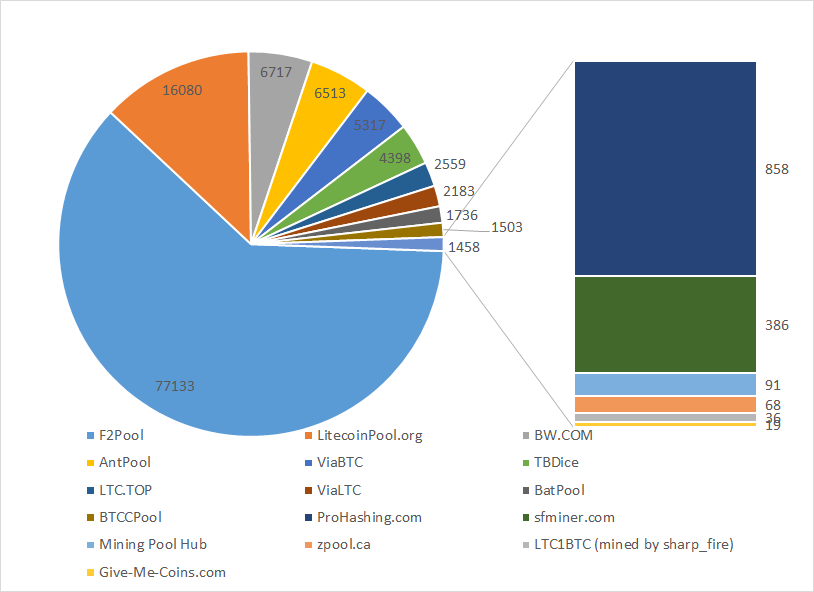
\includegraphics[width=1.0\linewidth]{images/distribuzionemining}
	\caption{blocchi per miner 2017, dati ottenuti tramite BlockAPI}
	\label{fig:distribuzionemining}
\end{figure}


\section{Merged Mining}
\subsection{Contesto}
Il merged mining, noto anche come Auxiliary Proof of Work, permette di minare contemporaneamente due criptovalute che utilizzino lo stesso algoritmo di hashing (Scrypt nel caso di Litecoin).
I calcoli vengono svolti e sfruttati per due blockchain, il che permette alle blockchain minori di aumentare il proprio potere di hashing. In questo caso il merged mining riguarda Litecoin e Dogecoin, entrambe criptovalute il cui mining è basato su Scrypt.
Ho identificato il pattern esadecimale [fabe6d6d] che viene inserito nella coinbase per segnalare che il blocco è frutto di merged mining.

\begin{figure}
	\centering
	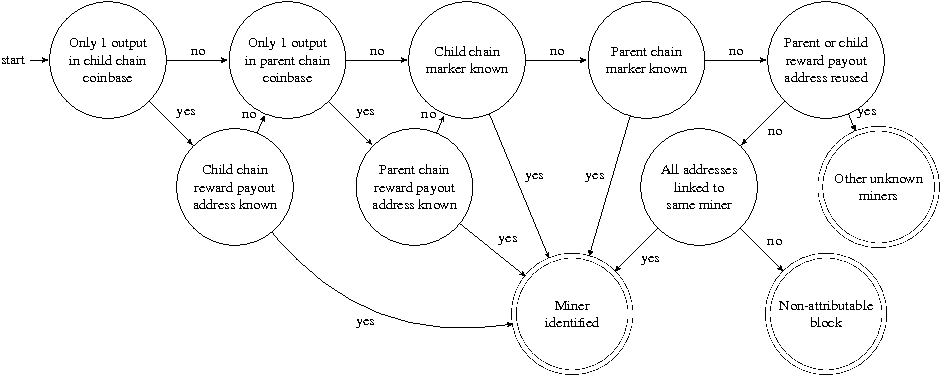
\includegraphics[width=1.0\linewidth]{images/mergedminingdiagramsemanticscholar}
	\caption{Funzionamento del merged mining, fonte Semantic Scholar}
	\label{fig:mergedminingdiagramsemanticscholar}
\end{figure}

\subsection{Obiettivo dell’analisi}
Identificare quanti blocchi vengano ottenuti tramite merged mining e chi li ha minati, la diffusione della pratica nel corso degli anni.
\subsection{Svolgimento}
L’esame dell’hex della transazione coinbase questa volta si orienterà sulla ricerca del pattern fabe6d6d. Ho effettuato l’analisi sullo stato dell’intera blockchain Litecoin fino al 02/08/2018.
\subsection{Query}

\begin{lstlisting}
SELECT COUNT(*) as "Blocks", isMerged as 'MM?' FROM myblockchainlite.ltcpools WHERE timestamp > "2018-01-01" AND pool != "unknown"
GROUP BY MM?;
\end{lstlisting}

\subsection{Risultati}


Nel 2018, 62046 blocchi su un totale di 63434 il cui pool è noto e/o rilevabile dal tool sono minati con merged mining. È il 98.37\%, da cui deduciamo che ormai la quasi totalità dei mining pools adotta questo sistema.


\begin{tabular}{|l|c|}
	\hline 
	\textbf{Year} & \textbf{MM\%} \\ 
	\hline 
	2014 & 31.29 \\ 
	\hline 
	2015 & 87.61 \\ 
	\hline 
	2016 & 98.27 \\ 
	\hline 
	2017 & 97.96 \\ 
	\hline 
	2018 & 97.82 \\ 
	\hline 
\end{tabular}
 
\begin{tabular}{|c|c|}
	\hline 
	\textbf{Blocks2018} & \textbf{MM?} \\ 
	\hline 
	1388 & No \\ 
	\hline
	62406 & Yes \\
	\hline
\end{tabular}


La figura \ref{fig:nomerged-vs-merged} mostra per ogni anno a partire dal 2014 (poiché i dati precedenti non sono significativi) la proporzione tra i blocchi frutto di merged mining e non.

\begin{figure}[h!]
	\centering
	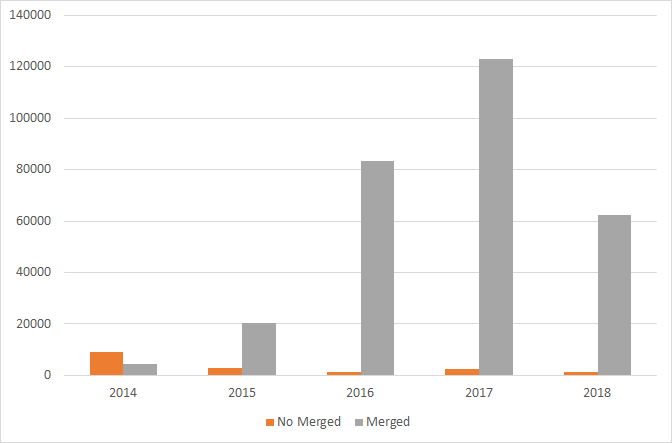
\includegraphics[width=1.0\linewidth]{images/nomerged-vs-merged}
	\caption{Proporzione tra blocchi minati con e senza merged mining. Dati ottenuti tramite BlockAPI.}
	\label{fig:nomerged-vs-merged}
\end{figure}


\section{Empty blocks}
\subsection{Contesto}
La generazione di un nuovo blocco comporta l’attribuzione della ricompensa al miner che trova la soluzione del cryptopuzzle in aggiunta alle fees, ovvero l’incentivo che l’autore di ogni transazione fornisce al miner per dare priorità all’inserimento di essa nel blocco.
Quando le fees sono trascurabili rispetto al guadagno immediato della reward, un miner (o mining pool) poco onesto può decidere di puntare unicamente alla soluzione del puzzle senza alcun impegno alla validazione delle transazioni, guadagnando così la ricompensa senza apportare nulla di utile alla blockchain. Ciò ha anche l’effetto collaterale di costringere indirettamente gli utilizzatori a ricorrere a fees più alte per fornire un incentivo ai miners per interessarsi alla transazione.
Il problema è più accentuato per le criptovalute la cui blockchain prevede una rapida generazione dei blocchi e fees mediamente basse come Litecoin.

\subsection{Obiettivo dell’analisi}
Verificare quanti blocchi vuoti vengono minati e se un particolare mining pool sta attuando sistematicamente questo comportamento.
C’è da attendersi risultati significativi da parte di mining pools con elevato hashing power.

\subsection{Svolgimento}
Ogni blocco Litecoin presenta sempre almeno una transazione coinbase, per cui si identificano i blocchi che contengono una sola transazione e chi li ha minati, se noto. Si può visualizzare, per ciascun miner, qual è il rapporto tra blocchi vuoti e non vuoti e dedurre da questo se siano casi isolati oppure segno che il pool sta attuando sistematicamente questo comportamento.

\subsection{Query}

\begin{lstlisting}
SELECT miner, COUNT(*) as emptyblocks 
FROM `emptyblockanalysis` where txsnumber = 1
GROUP BY miner
ORDER BY emptyblocks DESC;
\end{lstlisting}


Questa query conta quanti sono i blocchi vuoti minati da ciascun miner riconosciuto.

\begin{lstlisting}
SELECT miner,
COUNT(CASE WHEN txsnumber = 1 THEN 1 ELSE NULL END) AS emptyblocks,
COUNT(CASE WHEN txsnumber > 0 THEN 1 ELSE NULL END) AS totalblocks
FROM emptyblockanalysis
GROUP BY miner;
\end{lstlisting}

Tramite questa query si può confrontare il dato dell’analisi precedente, che di per sé ci dice poco, con il numero totale di blocchi che il miner in questione ha minato. Da qui possiamo evincere quali miner lo adottano come comportamento sistematico.

\begin{lstlisting}
SELECT t1.miner as BlockMiner,
t1.emptyblocks as EmptyB,
t1.totalblocks as TotalB,
t1.emptyblocks/t1.totalblocks as Ratio 
FROM ((SELECT miner,
COUNT(CASE WHEN txsnumber = 1 THEN 1 ELSE NULL END) AS emptyblocks,
COUNT(CASE WHEN txsnumber > 0 THEN 1 ELSE NULL END) AS totalblocks
FROM emptyblockanalysis
GROUP BY miner) as t1)
ORDER BY Ratio desc;
\end{lstlisting}		

Infine, questa query ci fornisce una vista ordinata in modo decrescente per ratio empty/total delineando meglio il quadro generale.				
\subsection{Risultati}

\begin{figure}[h!]
	\centering
	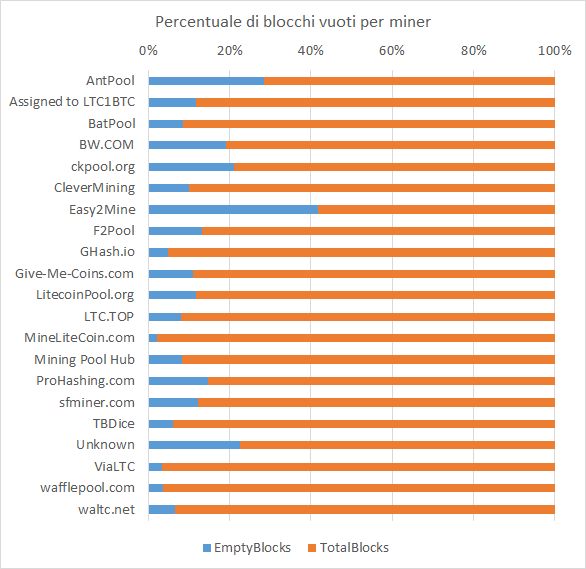
\includegraphics[width=0.8\linewidth]{images/percentuale-blocchi-vuoti-per-miner}
	\caption{\% di blocchi vuoti per i principali miners. Dati ottenuti tramite BlockAPI}
	\label{fig:percentuale-blocchi-vuoti-per-miner}
\end{figure}


Il grafico in figura \ref*{fig:percentuale-blocchi-vuoti-per-miner} indica, per ogni miner, qual è la percentuale di blocchi vuoti rispetto ai blocchi totali

Nonostante il bug citato nel cap 3.1 relativo ai mining pools che impedisce la corretta attribuzione di alcuni blocchi ai rispettivi miners, la percentuale di blocchi vuoti minati da AntPool, BW.COM e F2Pool tra quelli rilevati è visibilmente degna di nota. L’osservazione tramite un explorer esterno (nella fattispecie litecoinpool.org che sfrutta l'explorer chain.so) ha permesso di riscontrare che AntPool tende a minare anche svariati blocchi vuoti consecutivi, dimostrandosi sotto questo punto di vista uno tra i pools più negativi.
La distribuzione tra i mining pools sul totale dei blocchi vuoti riscontrati nella blockchain è riportata nella figura \ref{fig:distribuzione-blocchivuoti-ring}.

\begin{figure}[h!]
	\centering
	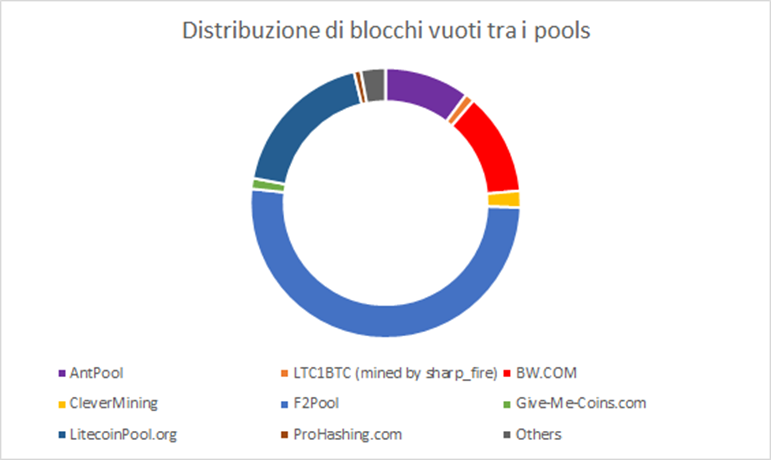
\includegraphics[width=1.0\linewidth]{images/distribuzione-blocchivuoti-ring}
	\caption{Ripartizione dei blocchi vuoti tra i pools. Dati ottenuti tramite BlockAPI}
	\label{fig:distribuzione-blocchivuoti-ring}
\end{figure}


\section{OP\_RETURN protocols}
\subsection{Contesto}
OP\_RETURN, di base, è uno degli opcodes del linguaggio Script. Rende la transazione non spendibile, per cui tutto ciò che viene inserito dopo esso non ha rilevanza e questo permette di allegare 40[80] bytes di dati arbitrari. Solitamente viene utilizzato per allegare un messaggio. Tuttavia, poiché la blockchain per ragioni di efficienza e spazio non permette l’inserimento di files allegati e la necessità di avere milioni di copie della blockchain rende impensabile l’implementazione di un servizio simile si sfrutta questo piccolo spazio per allegare in forma compatta un riferimento a dati esterni.
Tramite l’OP\_RETURN è possibile utilizzare servizi aggiuntivi che si appoggiano alla blockchain ma risiedono su un altro strato (layered network). Servizi di timestamping, firma digitale, archiviazione possono utilizzare la blockchain per includere riferimenti a dati residenti all’esterno di essa e marcare con il loro identificatore i primi 4 bytes dell’OP\_RETURN

OP\_RETURN è supportato su Litecoin a partire dalla versione 0.9: pur non avendo raggiunto una diffusione comparabile a quella conseguita su Bitcoin è stata comunque riscontrata la presenza di metaprotocolli nella blockchain, tra cui alcuni dei più noti che si appoggiano a Bitcoin stesso.
Recentemente l’OP\_RETURN è stato utilizzato per inserire un header indicativo dell’adesione a Segwit: quest’ultimo è un protocollo che nasce per ovviare ad un problema di scalabilità che riguarda la blockchain.

\begin{figure}[h!]
	\centering
	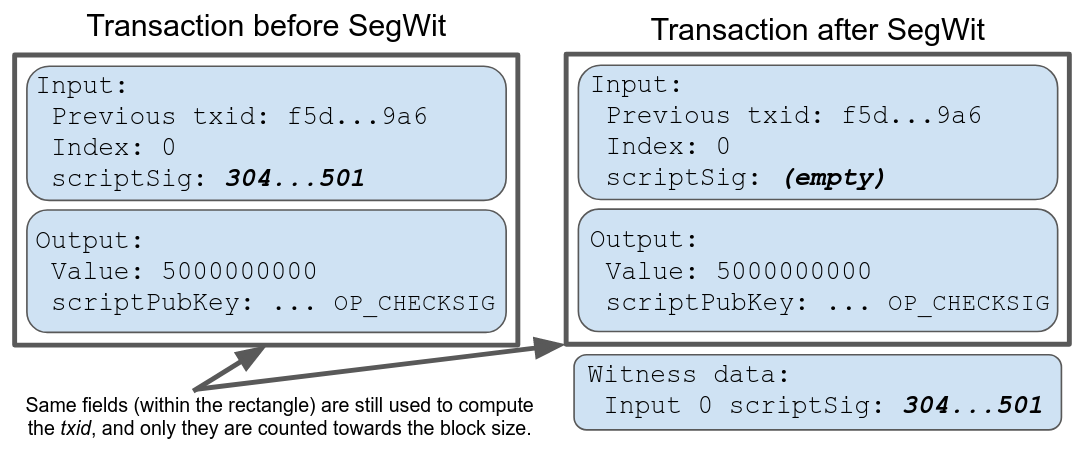
\includegraphics[width=1.0\linewidth]{images/before-after-segwit-medium}
	\caption{Transazioni prima e dopo SegWit (medium.com)}
	\label{fig:before-after-segwit-medium}
\end{figure}


Il problema si è posto con la crescita dell’interesse verso l’utilizzo delle Blockchain, in quanto ogni blocco di transazioni deve rispettare il limite massimo di 1MB e questo ha cominciato a causare congestione e ritardi sui network. Talvolta i tempi di attesa sono stati nell’ordine delle ore. Inoltre un rischio notevole per la sicurezza era rappresentato dalla malleabilità, ossia la possibilità che il destinatario intercettasse l’ID della transazione del mittente modificandola a suo favore. Queste ragioni hanno portato alla separazione (da qui Segregated) della firma digitale (Witness): i dati della firma digitale, che fino ad ora occupavano fino al 65\% dello spazio della transazione, sono ora separati e la transazione contiene un puntatore ad essi affinché il software possa trattare indipendentemente le due parti.


\begin{figure}[h]
	\centering
	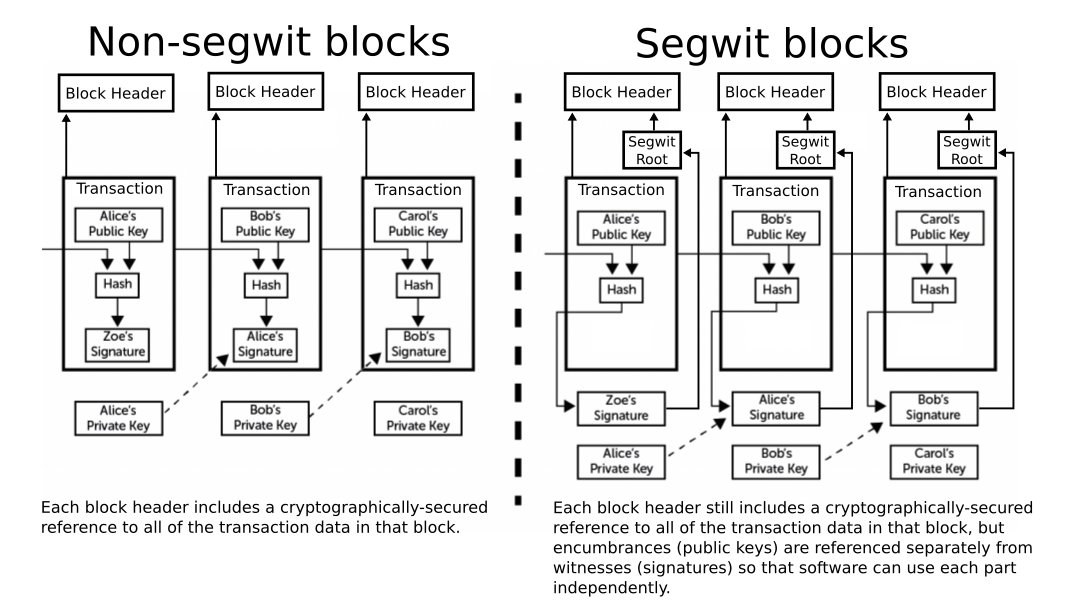
\includegraphics[width=1.0\linewidth]{images/segwitvsnonsegwit-medium}
	\caption{differenza tra blocco SegWit e non SegWit (medium.com)}
	\label{fig:segwitvsnonsegwit-medium}
\end{figure}


La condizione necessaria affinché il sistema SegWit funzioni è l’adozione da parte di almeno il 95\% del network e la segnalazione dell’adozione del sistema da parte dei miners è fondamentale per ritenere il consenso necessario all’implementazione del soft fork.


\subsection{Obiettivo}
Identificare tramite pattern noti i metaprotocolli utilizzati e l’header di adesione a SegWit.
\subsection{Svolgimento}
Si identificano le transazioni OP\_RETURN della blockchain. BlockAPI contiene una lista di pattern conosciuti utilizzati anche su Bitcoin ai quali ho aggiunto alcuni pattern scoperti tramite ricerca e consultazione dei siti ufficiali dei fornitori dei servizi.

\begin{figure}[h]
	\centering
	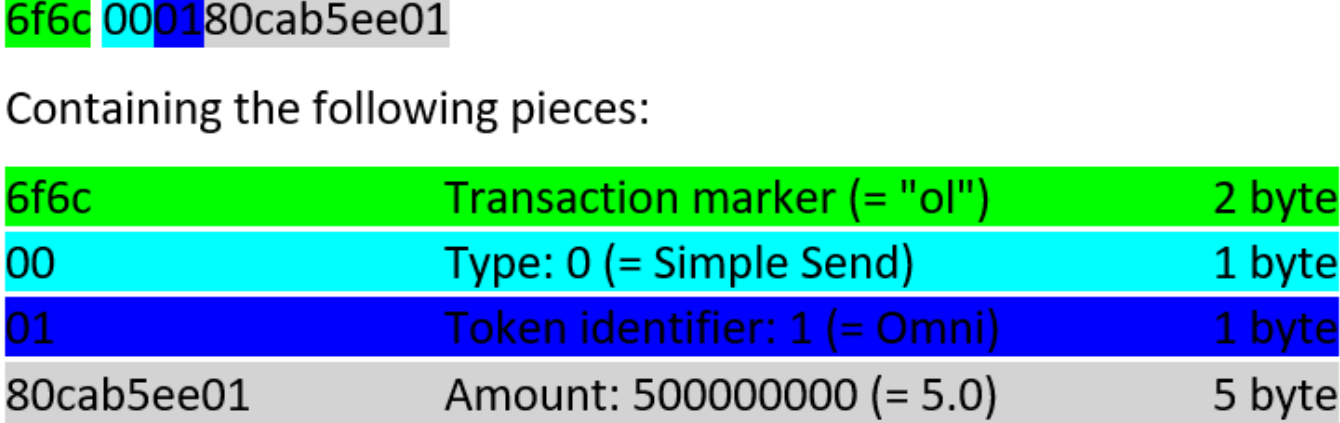
\includegraphics[width=1.0\linewidth]{images/ol-omnilayer-medium}
	\caption{Struttura di un OP\_RETURN di Omni Layer (medium.com)}
	\label{fig:ol-omnilayer-medium}
\end{figure}

Su ciascuna di esse, in modo analogo a quanto fatto sulle coinbase per l’analisi dei mining pools, si effettua un parsing dell’output tramite il seguente script:

\begin{lstlisting}
block.txs.foreach(tx => {
tx.outputs.foreach(f = out => {
if (out.isOpreturn()) {
var protocol: String =
MetadataParser.getApplication(tx.inputs.head.outPoint.toString.substring(0, 64), out.transOut.toString)
var metadata: String =
out.getMetadata()
\end{lstlisting}

Otteniamo i metadata della transazione.

\begin{lstlisting}
var segwit: Boolean =
MetadataParser.isSegwit(metadata)
\end{lstlisting}

Il Boolean ‘segwit’ restituisce true se l’OP\_RETURN rispetta la seguente struttura dichiarata sul github ufficiale:

\begin{tabular}{c|c}
	\textbf{Bytes} & \textbf{Funzione} \\ 
	\hline 
1 Byte	& OP\_RETURN (0x6A) \\ 
	\hline 
1 Byte	& Push dei seguenti 36 Bytes (0x24) \\ 
	\hline 
4 Byte	& Header SegWit (0xAA21A9ED) \\ 
	\hline 
32 Byte	& SHA256(SHA256(witness root hash|witness root value)) \\ 
	\hline 
39° e oltre	&  Dati opzionali non riguardanti il protocollo\\ 
\end{tabular} 

\begin{lstlisting}
outputTable.insert(Seq(tx.hash.toString, convertDate(block.date), protocol, metadata, segwit))
}
})
})
\end{lstlisting}
\subsection{Query}

SELECT protocol, count(*) as number FROM opreturn.opreturnoutputlite
group by protocol order by number desc;

Verifichiamo quante tra le transazioni contengono dei meta-protocolli a noi noti che si riferiscano a servizi layered.

\begin{lstlisting}
SELECT isSegwit as "Signaling Segwit?", Count(*) as TxNumber FROM opreturn.opreturnoutputlite
GROUP by isSegwit;
\end{lstlisting}

L’header della transazione “aa21a9ed” è un codice non-ascii che segnala l’utilizzo di SegWit nel blocco. Allo stato attuale dello sviluppo delle librerie di terze parti utilizzate per la blockchain Litecoin, non abbiamo a disposizione gli strumenti per effettuare ulteriori analisi sul contenuto dei metadati dell’OP\_RETURN il cui header segnali SegWit.
\subsection{Risultati}

Un primo conto significativo si può effettuare per dividere gli OP\_RETURN utilizzati allo scopo di segnalare SegWit da quelli utilizzati per qualsiasi altro scopo: come abbiamo detto è possibile utilizzarli per introdurre altri servizi esterni alla blockchain, ma anche per ancorare un messaggio in modo permanente alla blockchain seppur meno diffusamente di quanto accada su Bitcoin, nel quale la funzionalità viene sfruttata da molto più tempo.

\begin{tabular}{|c|c|}
	\hline 
	\textbf{Segwit?} & \textbf{TxCount} \\ 
	\hline 
	No & 24559 \\ 
	\hline 
	Yes & 234476 \\ 
	\hline 
\end{tabular} 

\begin{tabular}{|c|c|}
	\hline 
	\textbf{protocol}& \textbf{count}  \\ 
	\hline 
unknown	&  12381\\ 
	\hline 
copyrobo	&  7433\\ 
	\hline 
stampery	& 3577 \\ 
	\hline 
proofstack	& 967 \\ 
	\hline 
colu	& 69 \\ 
	\hline 
omni	& 67 \\ 
	\hline 
counterparty	& 35 \\ 
	\hline 
openassets	& 26 \\ 
	\hline 
blockstore	& 2 \\ 
	\hline 
empty	& 1 \\ 
	\hline 
proofofexistence	& 1 \\ 
	\hline 
\end{tabular} 

Esaminiamo ora gli OP\_RETURN utilizzati per uno scopo diverso dalla segnalazione di SegWit: approssimativamente il 50\% non denota l’utilizzo di un metaprotocollo specifico. Questo numero include OP\_RETURNs che contengono messaggi testuali, stringhe la cui decodifica non corrisponde ad alcun ascii, eventualmente codificati in base-64 o in altro modo, e infine protocolli a noi ancora non noti o di cui non è stato possibile trovare un riscontro affidabile sul web.
La diffusione dei vari protocolli nel restante 50\% è riportata nella tabella.

\begin{figure}
	\centering
	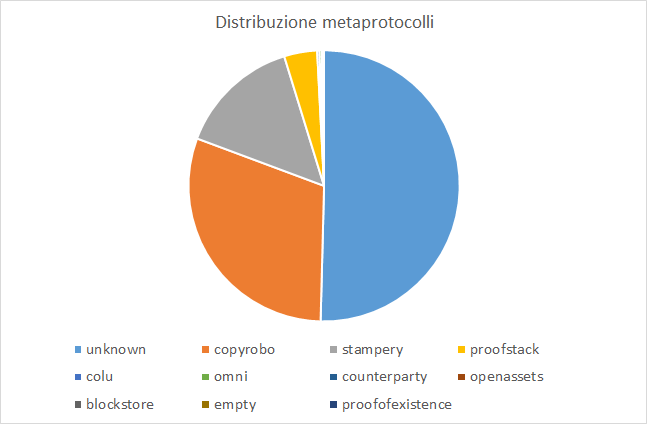
\includegraphics[width=1.0\linewidth]{images/distribuzioneopreturn}
	\caption{}
	\label{fig:distribuzioneopreturn}
\end{figure}



\chapter{Conclusioni e sviluppi futuri}

\section{Conclusioni}
Pur essendo nato nel 2011, il network Litecoin ha recentemente guadagnato valore ed attenzione da parte di investitori e sviluppatori. La crescita è stata esponenziale soprattutto negli ultimi due anni e l’interesse allo sviluppo software per la blockchain stessa e la sua analisi si sta solo ora avvicinando a quello di Bitcoin. Le sue caratteristiche lo rendono adatto a pagamenti elettronici e correntemente, dopo un tentativo con LitePay, la fondazione Litecoin sta valutando l’adozione di una carta di debito simile ad un bancomat per pagamenti “fisici”, per cui c’è da attendersi un incremento di interesse dal lato sia economico che software.
Seppur ancora distante dalla diffusione di Bitcoin si possono riscontrare in Litecoin diversi meccanismi comuni ad esso per via della similitudine tra i protocolli


\section{Sviluppi futuri}

Per quanto riguarda il tool, si può pensare sia ad un raffinamento delle analisi tramite adeguamento delle librerie già esistenti ai nuovi protocolli che all'implementazione di nuovi componenti per effettuare analisi analoghe a quelle che ho appena svolto su hard forks di Bitcoin come Bitcoin Cash. Quest’ultima seppur recente (nata il 1 agosto 2017) ha come obiettivo la riduzione delle fees e l’aumento della velocità di validazione delle transazioni sul network, ragioni per cui c’è da attendersi esiti e sviluppi simili a quelli di Litecoin.
Le tracce per il raffinamento delle analisi in un futuro prossimo sono tante: ad esempio il miglioramento delle API dei servizi web di terze parti, spesso ancora un po' carenti per Litecoin, e la maggior diffusione dei dati storici ad esso relativi permetterebbero analisi più accurate e significative riguardanti i bilanci, i tassi di scambio e le fees in relazione all'euro.

\subsection{Confronto con un lavoro correlato}
Il lavoro “Empirical Analysis of Crypto Currencies”\cite{relatedwork} mette a confronto gli ecosistemi Bitcoin e Litecoin ed esamina in ciascuno di essi il grado di correlazione tra transazioni input e output, e tra i top 100 indirizzi per ricchezza nelle due blockchain. Evidenzia che i più grossi tra i nodi sono miners e che in entrambi i casi i più ricchi tra di loro hanno scarsissima correlazione, il che evidenzia una maggior tendenza all’accumulo che alla spesa. Nel caso di Litecoin i $\frac{2}{3}$ degli indirizzi più ricchi risultano trasferire semplicemente i fondi da un account ad un altro tramite una piccola commissione.
L'autore misura inoltre il grado di clustering, ovvero i “triangoli” di transazioni a->b->a che possono indicare riciclaggio o semplici test di rete. Si tratta di un lavoro molto orientato alla statistica da cui si può trarre spunto per un'interpretazione in chiave statistica delle analisi già effettuate o di quelle future. 




\bibliographystyle{plain}
\bibliography{biblio}
\addcontentsline{toc}{chapter}{References}


\listoffigures

\listoftables	

\whitepage

\end{document}
